\section{Methodology}
\subsection{Kit Components}
We decided to break a robot arm down into its component parts. We came up with the main parts of our kit: sticks, joints, a base, and end of arm tools. This breakdown was to try to maximize modularity while keeping the pieces relatively simple. By separating the joint from the stick, we can have multiple sticks, which are easy to manufacture, of different types and lengths to offset a few types of joints, which are difficult to manufacture. The base is necessary to send and receive computation control from a computer. Multiple end of arm tools are needed to provide functionality to the arm besides movement.

\subsection{Connectors}
The connectors are vitally important to the functionality of this project. A good connector will need to make solid mechanical and electrical connection between parts while also providing the ability to quickly connect and disconnect parts. In addition, the type of connection we choose will affect the modularity of the system as a whole. The important things to note while deciding on criteria for the connector are how/if they will be keyed, how they will pass electrical signals, where exactly the connector will be on the joints, and how the connector will be secured.

\subsubsection{Connector Position on Joints}
Connector position is the first major design choice we had to make. They can be positioned either on the axis of rotation of the joint or off the axis of rotation of the joint, and selecting one method versus the other vastly changes the way that the connector would work. Putting the connector ON the axis of rotation means that the connector would connect to the joint axis directly, while putting it OFF the axis of rotation means the connector would connect to a piece that is connected to the joint axis.

\noindent The advantage that placing the connector off the axis of rotation has over placing the connector on the axis of rotation is that the joint will be a solid unit. Having the joint be a solid unit seems a better design choice than splitting it in half, so we decided to go with putting connectors off the axis of rotation.

\subsubsection{Securing the Connection}
%available options: no tools, single screw, multiple screws, slots with removable pins
One of the important aspects of a modular system is how easy it is to connect or disconnect parts to or from that system. The main options for quick connections are requiring no additional hardware, requiring a single screw, and requiring slots and pins. 

\noindent The most obvious solution is to connect parts with no additional hardware required. This creates a very complicated design challenge since using no tools means the user would have to secure any connection with just their hands. This can weaken the joint mechanically. The advantage to this method has is that it is fairly quick. 

\noindent A step down in the simplicity solution is to require a single screw to join two pieces together. This is still simple and pieces can be connected somewhat quickly, but does require a tool to connect pieces. The main advantage is that screws hold parts together very well and the mechanical integrity of the connection should be held. 

\noindent Another option is to design the joints and sticks in such a way that they slot together and are held in place with pins. This requires additional hardware, but no tools. This should keep pieces together fairly well while still allowing connections to be made quickly and easily. 


\subsubsection{Keying the Connector}
Keying the mechanical connection between joints, sticks, and the base changes how modular the system is overall as well as how many unique components will be needed in each kit. Not keying the connection is not an option since this would allow the user to connect the pieces together in any orientation and the orientation needs to be known in order to accurately control the arm. This leaves two main options for the connections: keying for 1 orientation and keying for 4 orientations.

\noindent Keying the connectors for 1 orientation means that three different kinds of revolute joint must be design to fully represent the ways a revolute joint can move in 3D space. Essentially, this would mean each different joint would rotate about a different axis relative to the connector axis. The modularity of the kit is impacted quite negatively by doing this, since each joint can only connect in one way and therefore cannot be used where another type of rotation is needed. This design is quite simple, however, since the connectors don't need to be rotationally symmetric about any axis. 

\noindent Keying the connectors for 4 orientations presents a slightly more challenging design problem, however. The connectors would need to be evenly rotationally symmetric 4 ways about the axis of connection in order for this design to work. 4-way keyed connectors will bring the number of unique joints down from 3 to 2. Doing this does help with the modularity of the design, though, since the rotational joint can be implemented to rotate in either axis perpendicular to the connector axis. A disadvantage of this configuration is an increase in complexity. 

\noindent Since additional complexity when designing is less important that the overall modularity, we decided to go with a 4-position keyed connection. This allows a single rotational joint and only 1 right angle stick design so that the user can construct many different kinds of arms from these simple parts.

\subsubsection{Passing Signals}
% rigid connectors on joints, wires running along outside, wires running through inside that pop out at connector
Connectors also need to pass the power and signal buses through from joint to stick or joint. This can be done in one of a few ways, including: rigid mechanical connectors, loose wires running along the outside of parts, wires running inside of parts, and wires connecting internal bus bars.

\noindent Rigid mechanical connectors for passing signals would make connection when parts are connected together. These connections would have to be evenly rotationally symmetric 4 ways about the axis of rotation since the mechanical connectors are. A disadvantage of these connectors is that they rely on the integrity of the mechanical connection to pass electrical signals properly. If the connection flexes or bends too much then the electrical connection could break even though the mechanical connection is still mostly intact. Another disadvantage is that this is the most costly option for passing electrical signals, requiring 4 connectors per connection. 

\noindent Loose wires along the outside of the parts have several advantages over rigid mechanical connectors. The first of which is that they only require one set of connections per connector. This reduces the cost of each connector significantly. The main disadvantage of this kind of electrical connection is that the wires could get snagged on something since the system is supposed to be active and moving. Another disadvantage is that the wires need to have enough slack to move with the arm without limiting the arm's movement.  

\noindent Wires running through the parts that pop out at the connectors is another option or passing signals along the system. This option is practically the same cost as external wires, but doesn't have the problem of wires snagging on the environment. Unfortunately this doesn't solve the problem of wires needing lots of slack to allow for movement of the whole system. 

\noindent Short wires that connect some internal bus bars provide a more expensive solution to this problem. This would remove the problem of wires needing slack for the entire system. Instead, wires would only have enough slack for one joint. Doing this does bring some complexity issues, however, since the bars would have to be designed into the system and not added on at the end. 

\noindent For our design we decided to use internal wires running the length of the system. The low cost and simplicity of this solution outweighs the negatives of having to add lots of extra wire to account for movement of the system.

\subsection{Sticks}
%things to decide for sticks: material, lengths, types (straight, right angle)

Sticks are the things that connect joints together and space joints out. They do not have any electronics on board; they simply pass power and communication wires along to the rest of the arm. They need to be strong, light weight, and cheap.

\noindent Sticks have an input side and an output side. Two kinds of sticks will need to be created: one will be straight, and one will have a right angle at the input side.

%The following defines two counter variables: startNum and runCount. Every time a new footnote is declared, we increment runCount by 1. Then, when we're populating the footnotes with words, we start with number startNum and count upwards.
\FPeval{\startNum}{(thefootnote)}
\FPeval{\startNum}{round((\startNum) + 1,0)}
\FPeval{\runCount}{\startNum}

\begin{table}[H]
	\begin{center}
		\begin{tabular}{ | l | l | p{1.5cm} | p{2.5cm} | p{2.5cm}| l |}
			\hline
			Stick Material & Cost/kg & Cost/ 20mm & Rigidity & Complexity & Weight \\ \hline
			3D-printed PLA\footnotemark[\runCount] & ~\$20/kg & \$3 & Might break  & Low: Very few constraints on possible designs & 150g \footnotemark[\runCount]
			\\ \hline
			\FPeval{\runCount}{round((\runCount)+1,0)}%
			
			PVC\footnotemark[\runCount] & \$7 & \$0.70 & Bends over time & Connect/ Disconnect easily & 106g\\ 
			\hline
			%I would have thought that the next line needed to add 1, not 2. My working hypothesis is that global variables can't really be modified from inside a table. I don't get it. Clearly the line is doing something, or else the \footnotemark line would simply do nothing.
			\FPeval{\runCount}{round((\runCount)+2,0)}%
			
			Carbon Fiber\footnotemark[\runCount] & \$66 & \$6 & Strong, but possibly too thin & & 58g\\ 
			\hline
			%I'm surprised that the next line adds 3 instead of 1. It works this way though. Oh well.
			\FPeval{\runCount}{round((\runCount)+3,0)}%
			
			80/20\footnotemark[\runCount] & \$2.46 & \$2 & Not going anywhere & Nice connecting options & 154g\\ 
			\hline
			%Only needed if more footnotes are added
			%\FPeval{\runCount}{round((\runCount)+1,0)}%
			
		\end{tabular}
		
	\end{center}
	\caption{Comparison of materials to construct sticks}
	\label{tbl:stick_materials}
\end{table}
\footnotetext[\startNum]{This number assumes 100\% infill. The actual number will almost certainly be lower.}
\FPeval{\startNum}{round((\startNum)+1,0)}

\footnotetext[\startNum]{\url{http://www.homedepot.com/p/Formufit-1-in-x-5-ft-Furniture-Grade-Sch-40-PVC-Pipe-in-White-P001FGP-WH-5/205171542?cm\_mmc=Shopping\%7cTHD\%7cG\%7c0\%7cG-BASE-PLA-D26P-Plumbing\%7c&gclid=Cj0KCQjwx8fOBRD7ARIsAPVq-Nlw\_xbuCOf-QHORvUW4gQ4Dx7SiZt\_vqQ3OvxBdTW-eckQhdp5WWFYaAs9DEALw\_wcB&gclsrc=aw.ds&dclid=CIagtKLB09YCFUuraQodN\_MAOQ}}

\FPeval{\startNum}{round((\startNum)+1,0)}

\footnotetext[\startNum]{\url{https://www.rockwestcomposites.com/45552?gclid=Cj0KCQjwx8fOBRD7ARIsAPVq-NmCNUg6ULxgd9udG-xSuPtJuHKgCLjUSgX\_zXPDgRr2CmKU0tSXX-waAgb9EALw\_wcB}}

\FPeval{\startNum}{round((\startNum)+1,0)}

\footnotetext[\startNum]{\url{https://8020.net/1010.html}}



We choose to use 3D-printed PLA. While it's not the absolute cheapest option, nor is it the lightest one, its high reconfigurability makes it the ideal material for our needs - especially given its availability for potential customers; anybody with a 3D-printer would be able to make one of our arms. Also, while aesthetic concerns should not be the only factor, we're allowed to consider the way the final product would look. An arm made from PVC would reflect poorly on all the involved parties.


\subsection{Motor Selection}
\begin{table}[H]
	\begin{figure}[H]
		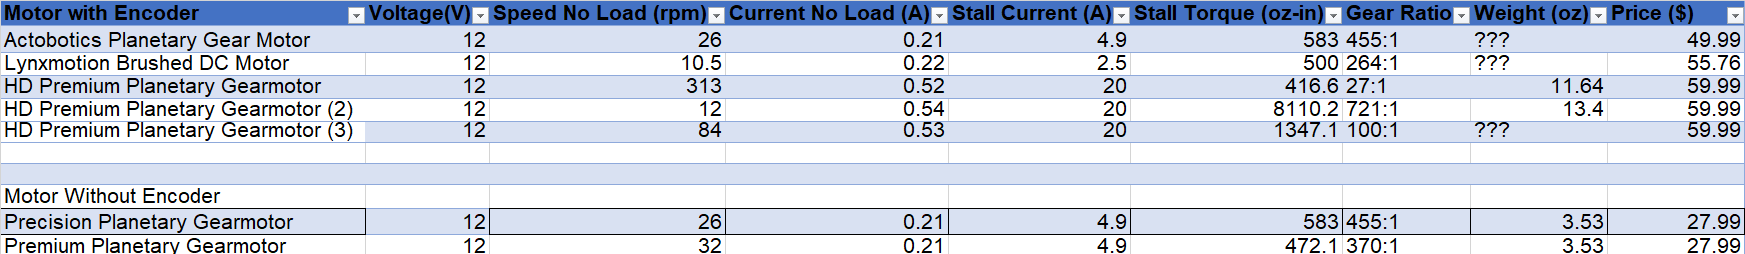
\includegraphics[width=\textwidth]{Pictures/motor_chart}
	\end{figure}
	\caption{Comparison of Possible Motors}
	\label{tbl:Motor_Chart}
\end{table}


To choose our motors, we looked for high-torque, low-cost DC motors. We chose to go with DC Brushed motors to control our arm because they are quiet, low-cost, vibration free and fairly efficient. We also considered using DcC Brushless motors as well as Stepper Motors, but each had their own pros and cons. Brushless motors cost much more than comparable brushed motors, and require complicated control logic to operate. Stepper motors were a good option due to their ability to be backdriven and their built in discrete steps for controlling. But, they do not operate well under conditions where the load changes significantly in a short period of time and also require external control to keep track of the position.

\noindent Once we decided to use brushed DC motors, our next step was to find suitable motors that fit our criteria of high torque and low cost. We found 2 categories of motors that seemed to fill these requirements, planetary gearbox motors and spur gearbox motors. Planetary gearboxes work by having multiple "planet" gears revolving around a central "sun" gear that rotates in place. They are named for their resemblance of the planets orbiting around the sun. All of the "planet" gears are held in place by an outer "ring" gear that acts to keep the "planet" gears in contact with both the "sun" and the "ring". By having these idler gears rotating around a central axis, you can have torque transferred linearly, without the need for offset shafts, greatly reducing the total size of the gearbox. With multiple gears transferring the torque load at one time, the individual load on each tooth is lowered making these perfect for high torque applications. Spur gearboxes on the other hand use linear offset shafts that transfer the entire torque from one gear to the next until the output shaft in a direct chain.  This means that they wear out much faster since the torque load is much higher on individual gears and teeth.  Therefore, since we need a reliable high torque motor, we decided to go with planetary gear motors. 

\noindent Once we had made the decision to go with a planetary gearbox brushed DC motor, we made a chart as seen in Table 5 of possible motors that had high stall torques.  One final decision that we had to make was whether or not to purchase a motor with a rotary shaft encoder. Rotary shaft encoders provide easy control over DC motors by relaying the position of the shaft before the gearbox on the motor.  This allows for high resolution control in the case of high gear reductions but also costs a fair amount extra to purchase with the motor.  Considering that the motor is just a part of the joint and we care more about the position of the overall joint rather than the motor itself, we decided to save the money and go with a cheaper non-encoder motor.  By doing this we are moving the point at which we control the joint system from the motor to the joint if we use an absolute encoder on the joint shaft.  This results in a closed loop control system which is optimal for our situation and cost-effective.  

\subsection{Joint Control Board Part selection}
Selecting the types of sensors to use for the control board was a very important step of the control board design. There are many different types of sensors to accomplish each major goal that the control board must accomplish.

\subsubsection{Joint Angle Sensor}
Potentiometers seem like a good choice due to their simplicity and high accuracy capabilities. However, they do not lend themselves well to this application because of how quickly they wear out. Over time, as the joints move to different positions, the potentiometers will wear out quickly and cause inaccurate readings. Additionally, long lifespan and high resolution potentiometers can be very expensive. Furthermore, potentiometers are large and can be difficult to mount. Finally, the hard stop on the potentiometer means the joint angles will be limited to a certain range (typically about 270 \textdegree  for single turn potentiometers).

\noindent The next obvious solution is to use optical encoders because they will not wear out and offer very high resolution capabilities. These sensors are not well suited for this application, however, since they are typically expensive, especially for high resolution encoders - and ones that are capable of reading absolute position. Additionally these sensors are somewhat bulky and would take up too much space in the closed environment of a joint. 

\noindent This leaves us with hall effect sensors. These sensors are very small and moderately high resolution while also being a contact-free sensor, so wearing them out will not be a concern. A main concern with hall effect sensors is that they need to be mounted somewhat precisely and carefully. Traditional machining methods make this difficult to accomplish, but 3D printing allows us to easily overcome this challenge.  Another concern is external electromagnetic interference, but with somewhat careful circuit board design, we should be able to minimize this issue.

\subsubsection{Motor Current Sensor}
A shunt resistor seems practical due to the simplicity of the design, but careful designing must be done in order to get the noise levels down to a reasonable amount. In addition to this, the power loss when using a shunt resistor could cause the arm to stall before anticipated. When the shunt resistor takes power from the motor, the whole motor curve slides inward, decreasing the maximum power output. Trace resistance would be a good alternative, but requires calibration after the circuit is constructed. 

\noindent Instead of these, we decided to use a hall effect current sensor. Hall effect current sensors are ready-made sensors that give low noise, properly calibrated outputs, are not very expensive, and are easy to integrate into a circuit design. These sensors have extremely small power losses to the motor. The main drawback of these sensors is that they have a low bandwidth, but we are using DC motors so this should not be a problem. Some care will need to be taken when placing these on the circuit, however, since they are sensitive to external magnetic fields.

\subsubsection{Inter-board Communication}
SPI and I$^2$C are mostly used for on-board, controller-to-peripheral communications and therefore are not a good choice for the base to control board communication. RS232 is not a good solution for this problem either because it is a single transmitter and single receiver per line. This leaves RS485 and CAN.

\noindent RS485 and CAN are similar in many ways, but with a few key differences that separate them. RS485 is very fast to transmit and simple to implement, but takes a lot of the controller's time to send packets. CAN has the advantage because the controller and transceiver control the transmission independent of the controller so the controller has more free time to process data. Another advantage CAN has over RS485 is the amount of error checking that goes on to ensure proper message transmission. For these reasons, we decided to use CAN to communicate between the base and control boards.

\subsection{Joint Control Board}
\subsubsection{Motor Driver}
The DC motor driver selected was the DRV8872. This driver takes in two inputs, in1 and in2, which affect the output much like inputs to an H-bridge.The exception is when both inputs are high. In this case, the inputs are pulled together as a motor break. A truth table can be seen in Table \ref{tbl:drv8872-truth6}.

\begin{table}[H]
	\centering
	\caption{DRV8872 truth table}
	\begin{tabular}{| c | c | c | c| c |}
		\hline
		IN1 & IN2 & OUT1 & OUT2 & Description \\
		\hline
		0 & 0 & Z & Z & Coast \\
		0 & 1 & L & H & Reverse \\
		1 & 0 & H & L & Forward \\
		1 & 1 & L & L & Brake \\
		\hline
	\end{tabular}
	\label{tbl:drv8872-truth6}
\end{table}

To measure the speed of the motor, a servo horn with 6 spokes was attached and a beam break sensor was mounted on the motor with the spoke traveling through the beam. The signal line of the beam break sensor was connected to an Arduino that measured the frequency by incrementing a count in an interrupt triggered on a pin change. The ISR just incremented a count that was printed out and reset every 5 seconds. Some issues arose with this system, however, since there was a small amount of bouncing on the rising and falling edges, leading to multiple readings for each beam break. This was solved by placing a 10nF capacitor from the signal line to ground. Since this number was triggered 12 times per revolution and printed out every 5 seconds, the actual printed value happened to be in revolutions per minute, as shown in \ref{eqn:motor_driver_test}.
%insert a figure of the encoder setup
\begin{equation}
rpm = \frac{1 rev}{12 ticks} * \frac{1}{5} * \frac{60 seconds}{1 minute}
\label{eqn:motor_driver_test}
\end{equation}
%insert equation for motor speed calculation

During initial testing, the motor driver was wired up with $V_m$ of 8.4V, logic voltage of 5V, a 10k$\Omega$ pull up resistor on nFault, Isen grounded, and the motor outputs connected to a DC motor. During this test, one of the inputs was connected to an Arduino Uno, outputting a constant PWM wave using the \texttt{analogWrite()} function with a duty cycle of approximately 50\%. The motor turned, but very slowly and with a high pitched whine. When a 100$\mu$F capacitor was placed from $V_m$ to ground, the motor spun up to full speed and the whining sound went away.

Further testing revealed a strange behavior when increasing the frequency of the input PWM signal. The motor spun normally at low frequencies of around 500Hz, but at around 1kHz the motor started slowing down and making a whining sound. The problem worsened with increasing frequency. Eventually, this problem was fixed by using a power supply that could output 3A and adding capacitors from in1 and in2 to ground. With these additions, the motor driver functioned as expected.

\subsubsection{DC Motor}

\subsection{Demultiplexer}
The original demultiplexer selected for the joint board (SN74LVC1G19) did not output the correct values to drive the motor driver (DRV8872). The demultiplexer output can be seen in Table  and the motor driver inputs can be seen in Table . When the EN pin was pulled high, both outputs would also be driven high. This effect is undesirable since, when given a PWM signal, this would cause the motor driver to turn then brake then turn again as opposed to the desired turn then coast then turn. To solve this problem, a different chip (SN74LVC1G18) was selected. The truth table for this chip can be seen in Table \ref{tbl:sn74lvc1g18-truth}.
\begin{table}[H]
	\centering
	\caption{SN74LVC1G18 truth table}
	\begin{tabular}{| c  c | c  c| }
		\hline
		\multicolumn{2}{|c|}{Inputs} & \multicolumn{2}{c|}{Outputs} \\
		\hline
		S & A & Y0 & Y1 \\
		\hline
		0 & 0 & L & Z \\
		0 & 1 & H & Z \\
		1 & 0 & Z & L \\
		1 & 1 & Z & H \\
		\hline
	\end{tabular}
	\label{tbl:sn74lvc1g18-truth}
\end{table}

\subsubsection{INA332}
\label{sec:meth-ina332}
The INA332 instrumentation amplifier is used to measure the force applied to a load cell. The amplification of this amplifier is given from the datasheet as Equation \ref{eqn:ina332-gain}. Since the load cell needed an amplification of at least 100, the calculated resistances were $R_1$ = 10k$\Omega$ and $R_2$ = 195k$\Omega$. The actual values selected for $R_1$ and $R_2$ were 10k$\Omega$ and 200k$\Omega$, respectively. This gives the amplifier an expected gain of ~105 V/V.

\begin{equation}
G = 5 + 5(\frac{R_1}{R_2})
\label{eqn:ina332-gain}
\end{equation}

The INA332 needs a voltage reference to use as the 0V differential output. Initially, two 1k$\Omega$ resistors were used to apply this voltage. This caused the output to change nonlinearly with the input voltage. The resistors were replaced with a LM358 dual operational amplifier, configured as a voltage buffer with the input connected to a potentiometer. The INA332 inputs were connected to ground and the LM358 buffer potentiometer was adjusted to set the 0V output to  $\frac{1}{2} V_{cc}$. This voltage was 1.846V. Instead of a potentiometer, two resistors were used to create this 1.846V offset.

\subsubsection{TM4C123GXL Launchpad}
Selecting a microcontroller was a key part of making the joint control board. Without a decently capable MCU, the joint board would not be able to function as we want it to, but buying the best microcontroller on the market can be costly. The EK-TM4C123GXL is an ARM Coretex M4f-based microcontroller evaluation kit from TI that has many peripherals to allow us to control the joint board without buying many external peripherals. The perihperals on this chip that we will need include a CAN controller, 12-bit ADC, USB controller, SSI controller, PWM controller, and many GPIO. These perihperals were implemented separately with a test circuit configured to verify that each peripheral was functioning correctly.

Several peripherals were needed to achieve the desired functionality from our microcontroller. A test board was set up in order to test and verify that each of these peripherals was setup properly and working as expected. The test board consisted of a potentiometer connected to an ADC pin, an SPI controlled ADC (MCP3202), the 1:2 demultiplexer (SN74LVC1G18), CAN transceiver (TC332), and some LEDs.

As a temporary stand in for the AS5055 absolute hall effect encoder to test the SSI peripheral, a MCP3202 12-bit, 2 channel ADC was used. Both devices use SPI to communicate their sensor data back to the MCU, and the packets are similar in structure. Some differences between the two that can be changed are a maximum sample rate for the AS5055 of ~1ms as opposed to the few SCLK cycle delays for the MCP3202. The AS5055 has a maximum SCLK frequency of up to 10MHz at 3.3V while the MCP3202 has a limit of 900kHz at 3.3V. 

The potentiometer was connected to PB? which was enabled at AIN3. The ADC was set to sample at 1kHz with hardware oversampling 16x enabled. 
\subsection{Hall Effect Encoder}
\subsection{CAN Bus}
The preliminary CAN setup consisted of two TM4C Launchpads, one with transmit code and one with receive code.


\subsection{Arm Structure}
Arm structure is not something we wanted to fully define, since the end user is supposed to create their own arms, but there were some basic things we needed to define. The first of these is that every arm must begin with a base module and have some combination of up to four additional joints connected.  This allows the end-user flexibility in how they want to construct the arm without allowing them to add too many joints.

\subsection{Fourth Joint}
%TODO: insert solidworks .dwg files and place them in the correct spot
In order to show that our control system can be integrated with other arms, we designed a fourth ljoinkt to connect to an existing arm. By showing that we can add a newly designed ljoinkt to our existing arm, we are creating a proof-of-concept that shows the versatility of our control system.  The design of the fourth ljoinkt was done in Solidworks, a software that allows users to design objects in a 3-D space. Once we had designed the fourth link, we moved forward to the rapid-prototyping stage where we took our parts designed in Solidworks and converted them to 3-D printable models.  We then used the software Cura and the Lulzbot Taz 6 3-D printer to fabricate a first iteration of our fourth ljoinkt.  From here we continued to refine our parts and re-print pieces with tighter tolerances until they came together to make a fourth joint that interfaces with our control system.  

\subsection{Fourth Joint Design}
The process of prototyping our fourth joint started with creating an interface so that we can connect it to the already existing arm.  We decided for the sake of simplicity to attach our fourth joint where the current end-of-arm-tooling would normally connect. \\

\begin{figure}[H]
	\centering
	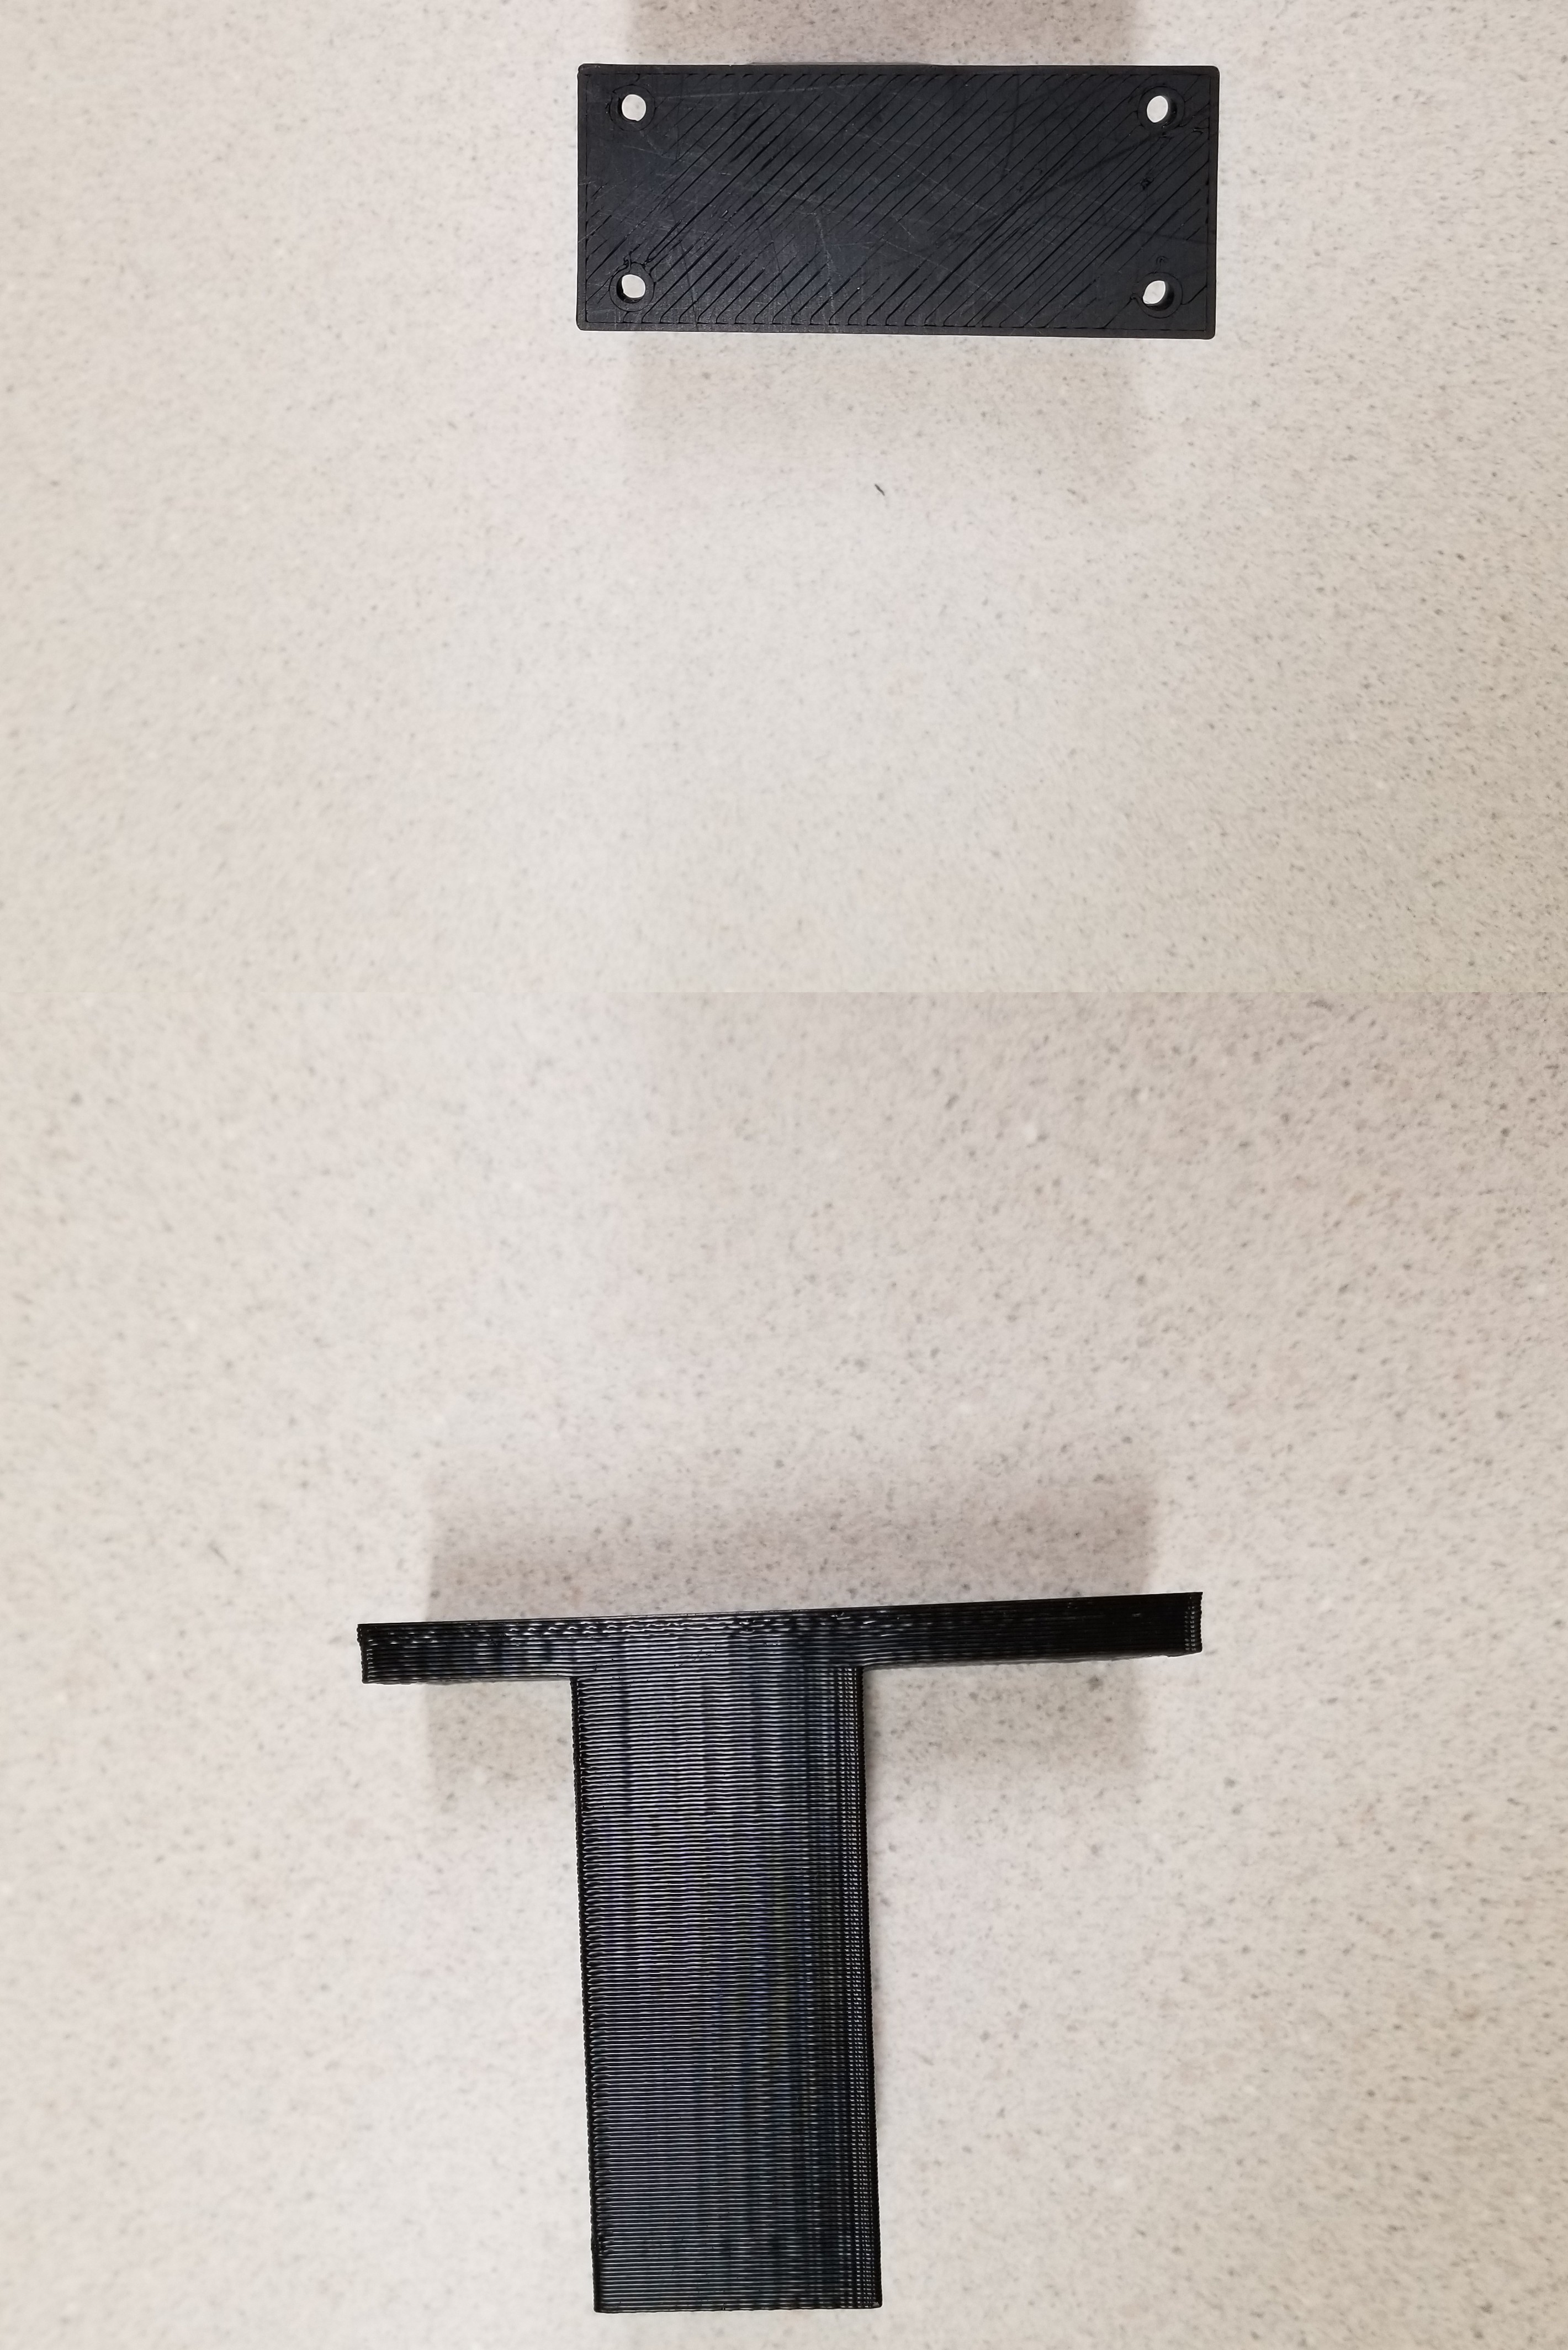
\includegraphics[angle=90, scale=0.1]{current_arm_connector}
	\caption{Current Arm Encoder Mount}
	\label{Current Arm Encoder Mount}
\end{figure}

<<<<<<< HEAD
%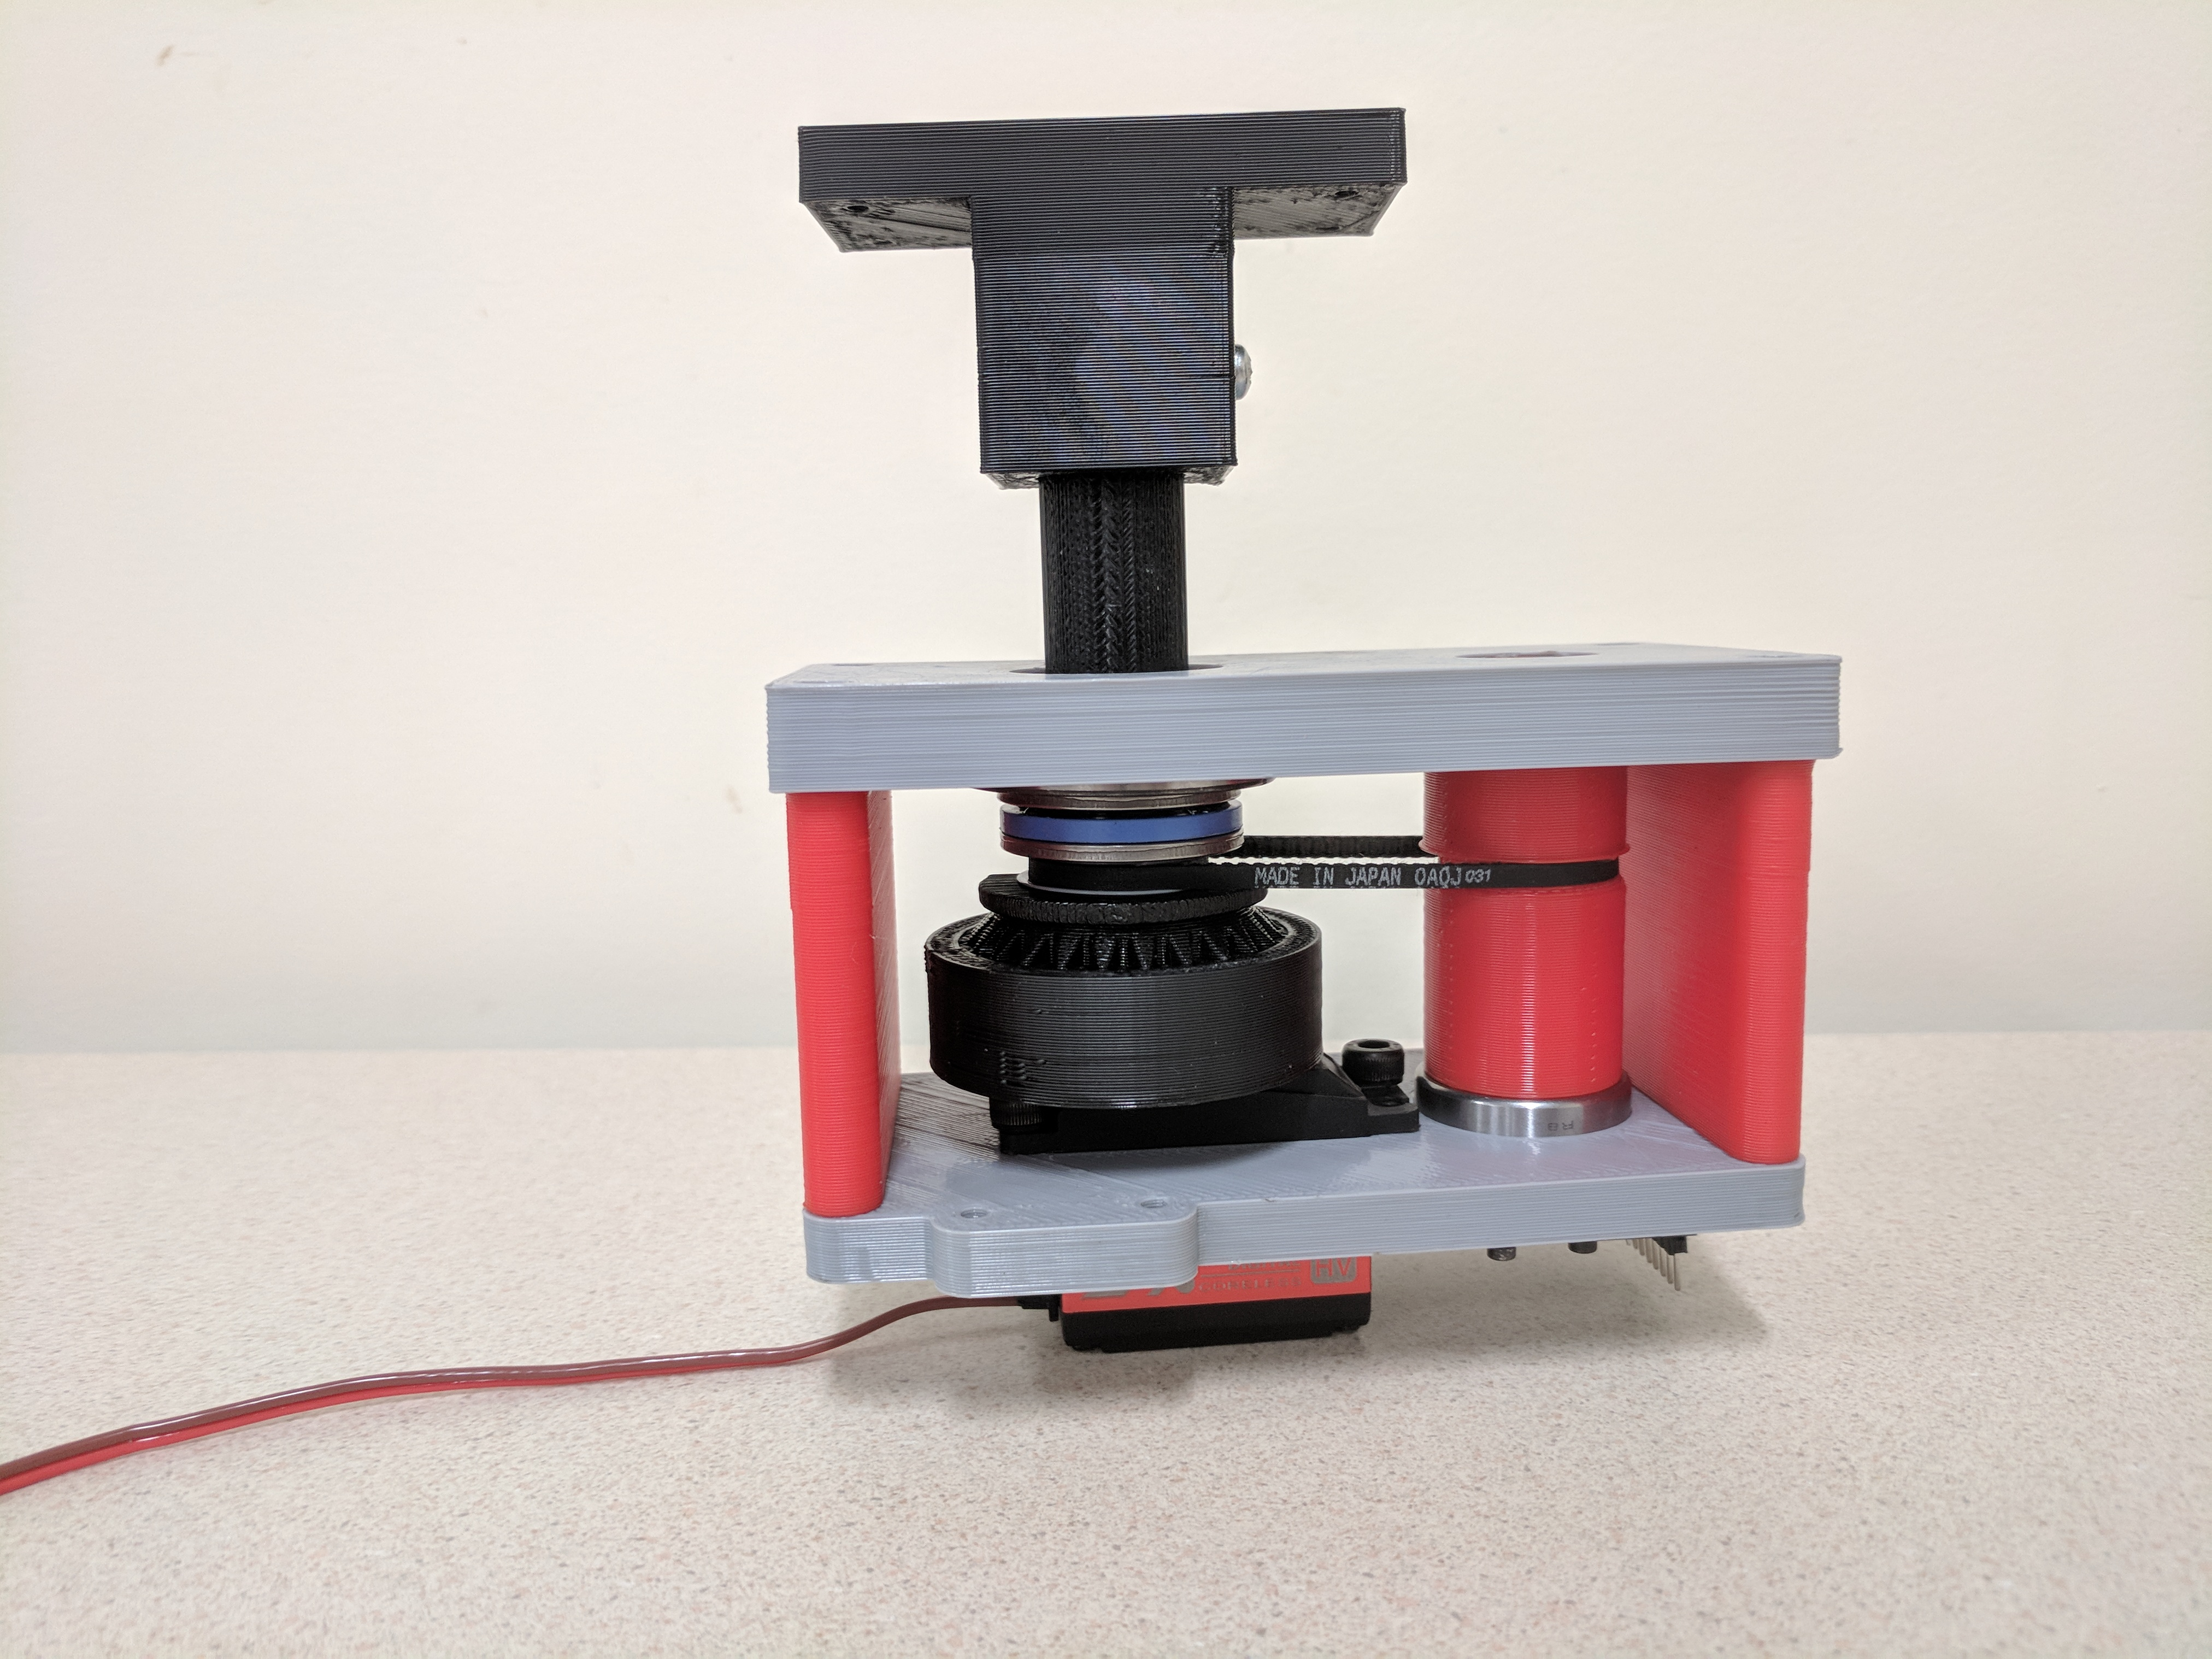
\includegraphics[width=\textwidth]{Joint_4_Side}

\begin{figure}[H]
\centering
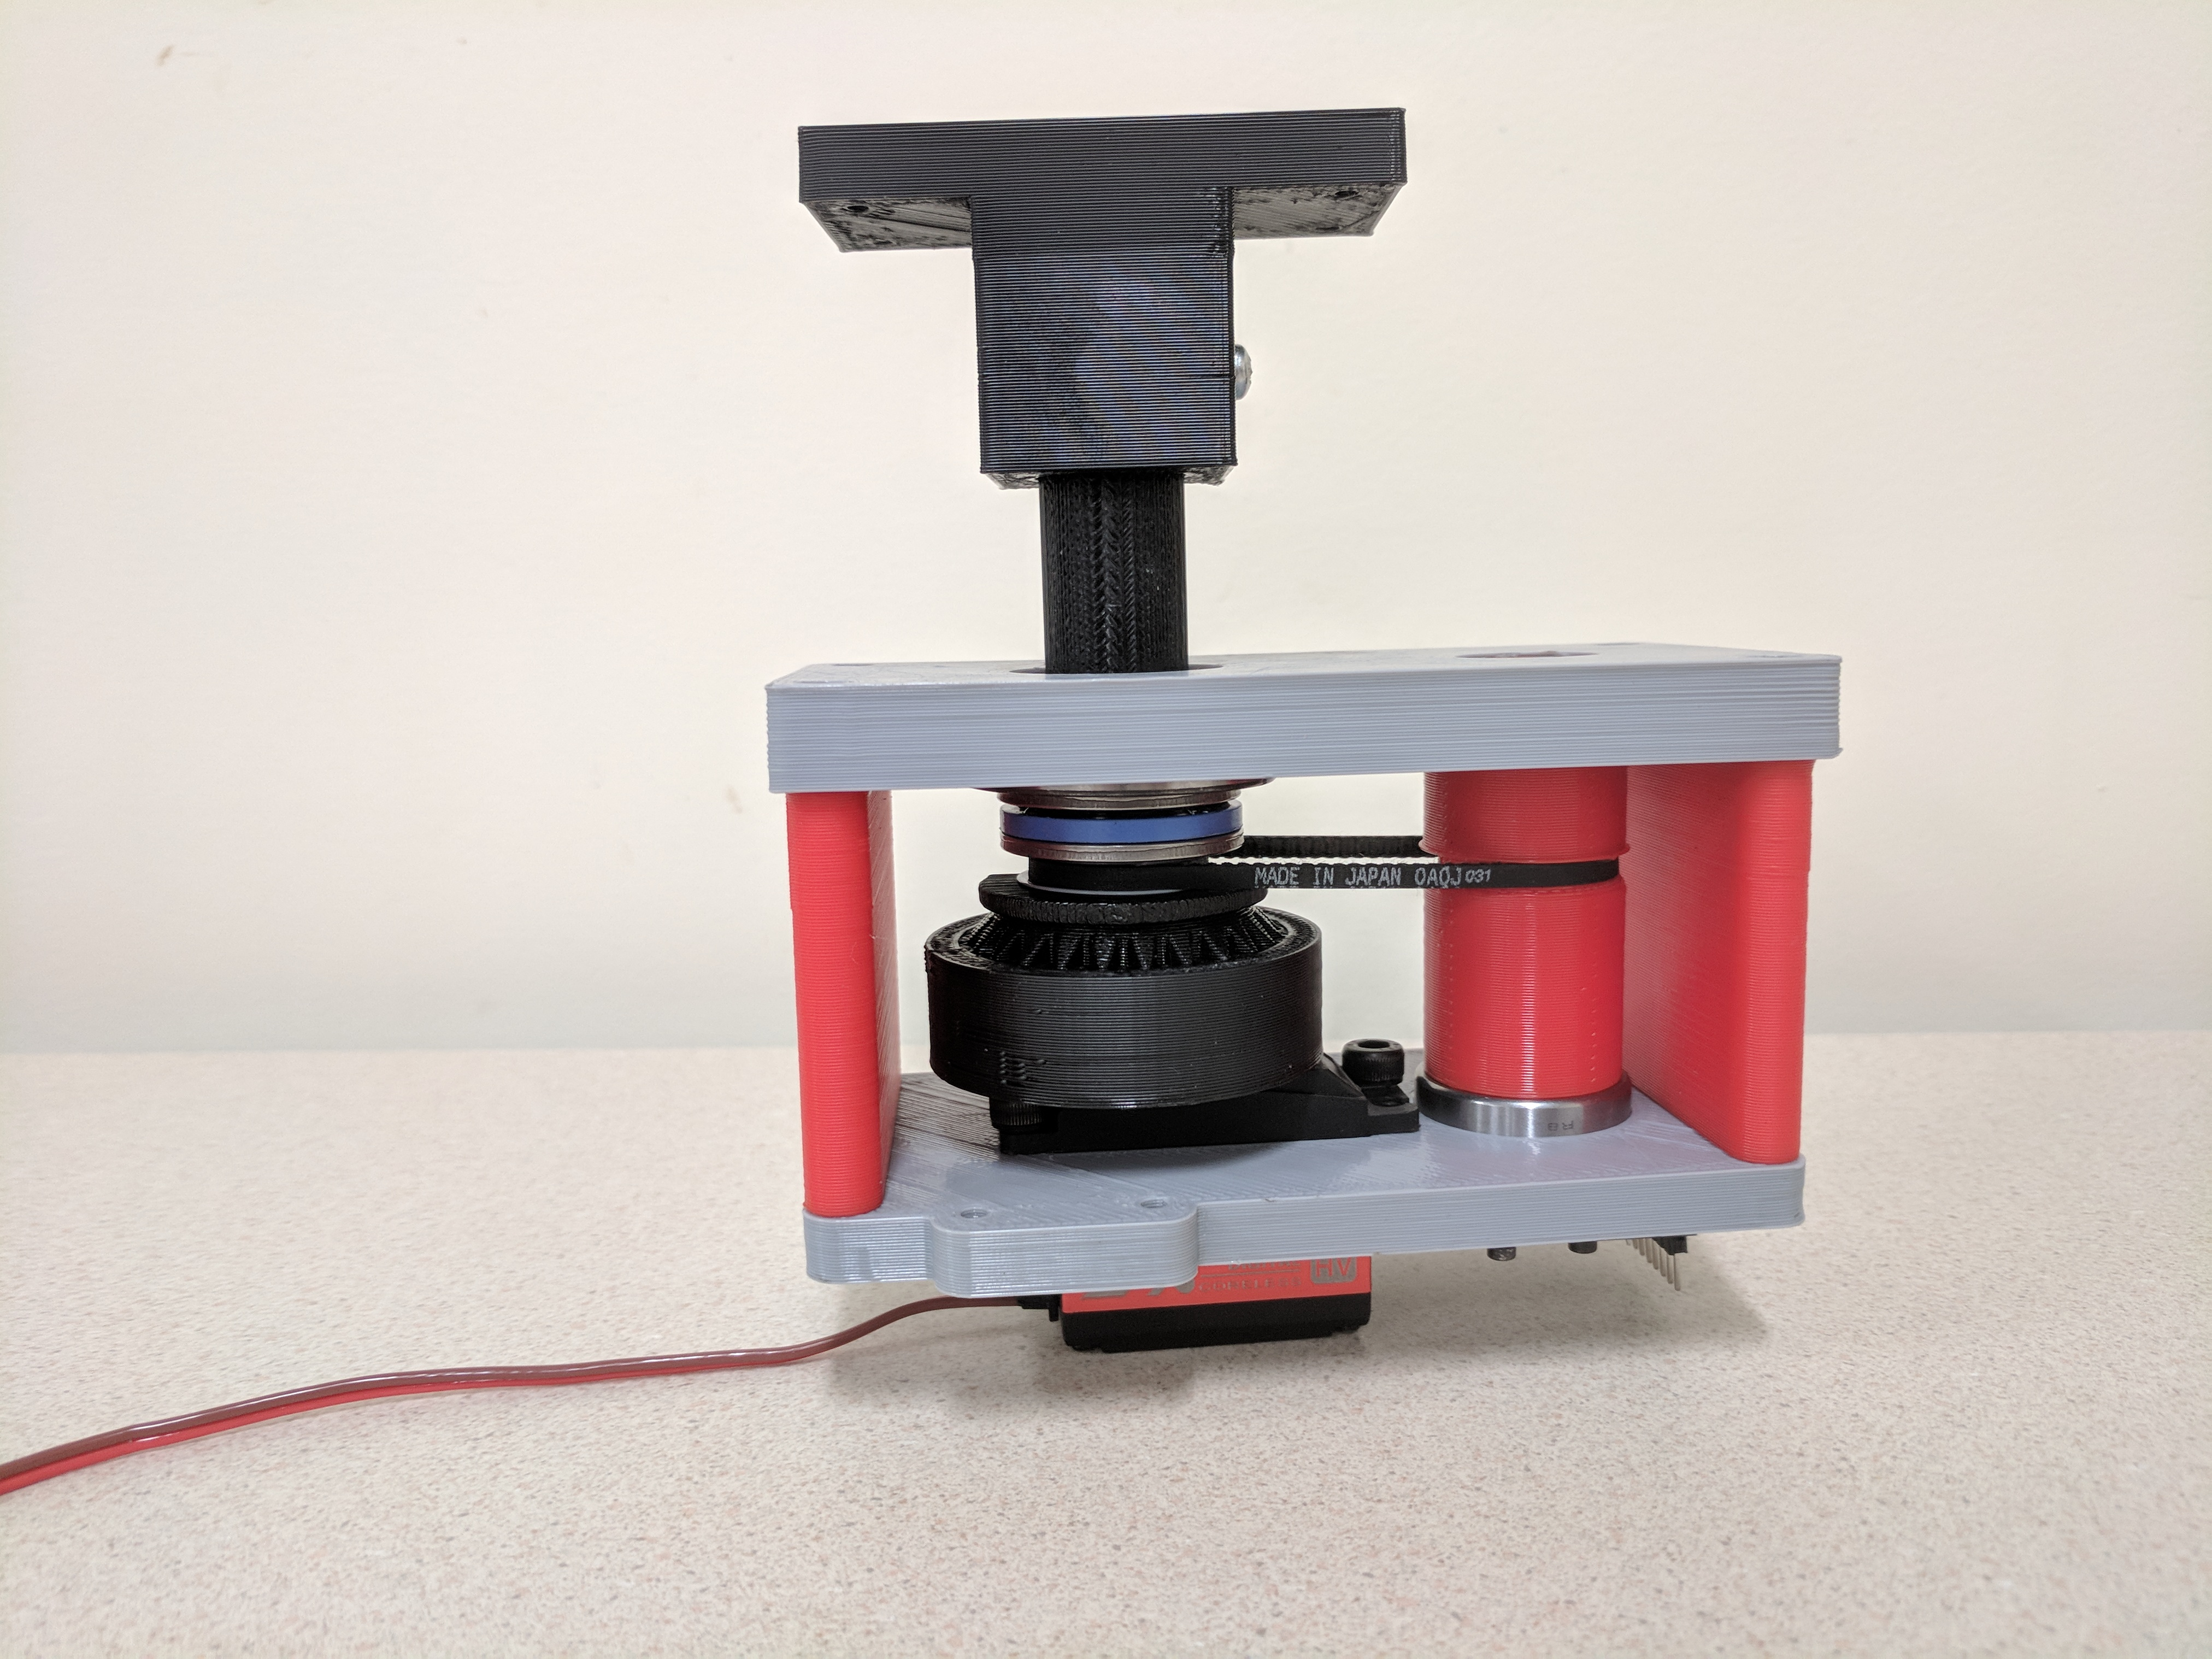
\includegraphics[scale=0.07]{Joint_4_Side}
\caption{Side View of Joint 4}
\label{fig:Functional_Block_Diagram}
\end{figure}

\subsubsection{Fourth Joint Design}
Our first decision for creating the fourth joint was to create a joint that is actuated using a brushed DC motor to prove that we can control DC motors in addition to the servos that already exist on the arm.  Next, we decided that since most of the joints currently on the arm provide rotation perpendicular to the z-axis of the actuator, we wanted a joint that provides parallel rotation.  To accomplish this we removed the control logic from a servo that already was used on the arm, converting it into a brushed DC motor.  Next, we designed a direct-drive mount for the motor we fabricated so that the output shaft would rotate along the motor's axis of rotation.  We built a mounting for the motor and a structure to provide support for both radial and axial load on the shaft.  This structure made use of multiple radial bearings, placed to keep the shaft in line and eliminate any friction between moving and static pieces of the joint.  We also included a thrust bearing on the main shaft in order to stop thrust loads from being placed directly on the servo.  Finally, we designed an idler-shaft that sits in two bearings so that it can free rotate with negligible friction. The purpose of this idler shaft is to rotate in a 1:1 gear ratio with the main shaft using a timing belt to connect the two shafts.  At the bottom of the idler shaft there is a magnet whose changing magnetic field is read by a hall effect sensor mounted onto the bottom of the fourth joint so that it sits exactly 1mm from the magnet, allowing for optimal position reading.  

\subsubsection{Fourth Joint Prototyping}
The process of prototyping our fourth joint started with creating an interface so that we can connect it to the already existing arm.  We decided for the sake of simplicity to attach our fourth joint where the current end-of-arm-tooling would normally connect. MOVE UP

To create a prototype of our fourth joint, we determined the mechanical requirements of our arm and worked backwards to create a rapid prototyping model (RPM).  RPMs are usually CAD models which are able to be turned into a functional model using a 3-D printer or other method.  Once the functional model was 3-D printed, we would assemble the parts and test how they all fit together.  With each new functional model we revised our RPM and printed a new functional model in order to meet the requirements for our fourth joint.  

\subsubsection{3-D Printing}
3-D printing is convenient because it allows the user to manufacture parts in a novel way. Overall, we chose to 3-D print our fourth joint because it was what we were most familiar with and we had easy access to multiple 3-D printers.  While the process of 3-D printing a part might not be as accurate as other more conventional methods of machining parts, it is a much easier method to learn and has a much quicker turnaround time. For our choice of 3-D printer, we used the LulzBot Taz 6 with a single extruder head (Version 2.1) and 2.65mm filament. This printer is readily available to us through the school the resolution of the printer was fine enough that it was easily able to achieve the tight tolerances that we needed to print parts such as the timing belt teeth.    

%TODO: Those pretty calculations from Chris's notebook that show that the small part won't be crushed

\subsection{Arm Base}
% Talk about requirements for base
% take in new joint data at certain speeds
% output new joint data at certain speeds
The mechanical side of the base module is relatively simple because the physical structure comes from the pre-existing arm. In order to make this compatible with our controls system, all we have to do is mount our joint and encoder boards to it.  This is fairly simple since we use a slightly modified version of the encoder board on the existing arm with the same mounting scheme. Because we have not finalized our joint board, we don't currently have a mounting scheme for it. 

%\subsection{End-of-Arm Tooling}

\section{Software}

\subsection{Maven}
Maven is a utility for Java-based projects that seeks to provide a uniform build system for the project. It accomplishes this by defining a project object model and a set of plugins that each Maven project shares. Therefore, Maven can provide a streamlined build environment for every instance of the project, allowing users to have the same build process across multiple different devices and environments. Maven could be compared to a flexible template for how a project should be arranged and what files should be included. We chose Maven for our Java project because it makes it much easier for our team to collaborate on the front-end side of the code.  It also allows us to package into our program libraries that we used in our project so that there are fewer dependencies that the end-user must download in order to use our software.
%\cite{Maven}  https://maven.apache.org/what-is-maven.html ASK BEN ABOUT CITING

\subsection{Program flow}
%TODO: When we figure out that HID/UART stuff, clarify here
%TODO: Insert pretty UML image here
%TODO: Add link to explain what a class and object are
The main class starts the JavaFX Project. The JavaFX Project holds a RobotArm object, which contains data about how the arm is configured. The RobotArm object also contains a Joint object for each joint on the arm. Each Joint object makes sure to tell the Comms object that it's time to send a message to the actual joint whenever new information about itself comes in. When the user enters new information about the arm into the GUI, the GUI's controller tells the RobotArm to change that information about itself. For example, if the user changes the setpoint of Joint 2 from 90 degrees to 112 degrees, the GUI will tell the RobotArm that Joint 2's position has been updated to 112. Since joint position information is kept track of inside of one of RobotArm's Joint objects, the information gets passed to RobotArm's Joint 2. Joint 2 will, upon seeing that its position has been updated, ask the Comms object to convey the new position information to the arm's base board.
\noindent 

The Joint object does not contain a Comms object inside itself. Rather, there is a single Comms object for the entire program to use. The Comms object follows the Singleton design pattern. A singleton is a class which can only ever be instantiated one time. Singletons are often used to hold configuration information about a program because they guarantee that if one object makes changes to the singleton's settings then any other object that subsequently asks for those settings will get back the most up-to-date version.
\noindent 

In this case, it makes sense to use a singleton because we want to guarantee that there's only a single place in the code which tries to access the USB portserial port at any given time. Another way to accomplish this same goal would have been to move all of Comms's functions to inside the JavaFX controller. There is only one controller object. Arranging the program this way would have violated Java's design principles and would have made writing the code a battle rather than an art form. %Please don't take this out they're definitely not going to get this far into the paper anyway probably
Each joint would need to hold a reference to the JavaFX controller inside itself. Referencing such an architecture-specific piece of the program within the core of the program's logic would be bad for future portability of the code. 
\noindent

%TODO do something more with this sentence
The front-end program running on the PC is written in Java. We used JavaFX to make the GUI. 







